\documentclass[a4paper]{scrartcl}

%support for german language
\usepackage{polyglossia}
\setmainlanguage{german}

\usepackage{fontspec}
\usepackage{csquotes}
\usepackage{tabularray}

\usepackage[hidelinks]{hyperref}

%including external figures
\usepackage{graphicx}
\graphicspath{{figures/}}

%generation of plots and images
\usepackage{tikz}
\usepackage{pgfplots}

% packages for use while writing presentation, later no longer needed
\usepackage{todonotes}
\usepackage{blindtext}

% package for improved math handling and units
\usepackage{amsmath}
\usepackage{mathtools}
\usepackage[math-style = ISO, bold-style = ISO]{unicode-math}

\usepackage{siunitx}
\sisetup{locale = DE, per-mode = symbol}
\DeclareSIUnit{\samples}{Samples}

% Literaturverwaltung
\usepackage[backend=biber, style=alphabetic]{biblatex}
\addbibresource{literature.bib}

\author{Mirko Schultheiß}
\title{Auslegung eines DCF77 Empfängers}
\subtitle{Konzeption des Analogteils}


\begin{document}

\maketitle
\clearpage
\tableofcontents
\listoffigures
\clearpage
\section{Abstract}
In diesem Dokument soll der Analogteil eines möglichen Empfängers für das DCF77-Signal ausgelegt werden.
Zu diesem Thema wurde bereits viel Forschung betrieben.
Deshalb handelt es sich hier eher um einen einfacheren Empfänger, der dazu dienen soll, wichtige Elemente eines solchen Empfängers für Einsteiger in das Thema besser zu verstehen.
Die Quellencodierung des Signals wird nur am Rand erwähnt, ebenso wird die Demodulation aufgrund der niedrigen Trägerfrequenz komplett in den Digitalteil verlegt.
Dementsprechend lassen sich die Konzepte aus diesem Dokument ebenfalls auf andere amplitudenmodulierte Signale in einem ähnlichen Frequenzbereich anwenden.

\section{Grundlegende Information zu DCF77}

DCF77 ist ein Signal, welches von der Physikalisch-Technischen Bundesanstalt, kurz PTB, erzeugt wird. Es dient dazu, eine Standardfrequenz und die gesetzliche Zeit zu verbreiten.
Ausgesendet wird das Signal im Auftrag der PTB durch die Media Broadcast GmbH in Maiflingen südlich von Frankfurt und ist in weiten Teilen Zentraleuropas empfangbar.
Das ausgesendete Signal hat eine Frequenz von \qty{77.5}{\kHz} und ist in der ITU Frequenzliste mit einer Bandbreite von \qty{2.4}{\kHz} eingetragen.
Die Informationen zur Zeit sind der Trägerfrequenz per Amplitudenmodulation überlagert.~\cite{piester_zeit-_2004}

\subsection{Codierung der gesetzlichen Zeit}
Minuten, Stunden, der Kalendertag, der Wochentag, der Monat und das Jahr werden jeweils BCD-kodiert. Nach den Minuten, den Stunden und den Datumsinformationen wird jeweils ein Paritätsbit angehängt, mit dem auf Fehler in der Übertragung geprüft werden kann. Vor den Minutendaten werden einige Informationsdaten, wie die Ankündingung von Sommerzeit oder Schaltsekunden kodiert. Davor werden in den ersten \qty{14}{\s} Daten des Dienstleiters Meteo Time übertragen. Das genaue Kodiersschema ist in Abbildung~\ref{fig:timecode} dargestellt.

\begin{figure}[h!]
    \centering
    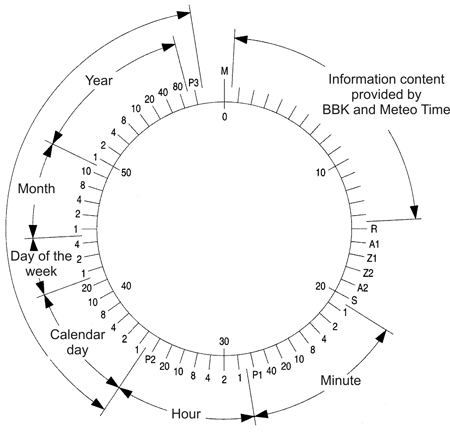
\includegraphics[width=0.7\textwidth]{timecode}
    \caption{offizielles Kodierschema des PTB~\cite{piester_time_2011}}
    \label{fig:timecode}
\end{figure}

\subsection{Modulation}
\label{sec:modulation}
Zu Beginn jeder Sekunde mit Ausnahme der 59. Sekunde einer Minute wird die Amplitude des Signals auf \qty{15}{\percent} abgesenkt.
Für eine \num{1} wird das Signal für \qty{200}{ms} abgesenkt, für eine \num{0} wird die Amplitude für \qty{100}{\ms} abgesenkt.
Auch wenn diese Art der Modulation von offizieller Stelle als Amplitudenmodulation beschrieben wird~\cite{piester_time_2011}, scheint dieses Modulationsschema sich besser als Puls-Weiten-Modulation (PWM) beschreiben zu lassen.
Zusätzlich werden der Trägerfrequenz per Binary Phase Shift Keying mit Pseudo-Random-Noise Sequenzen um \qty{\pm 13}{\degree} aufmoduliert, durch welche ein noch exakteres Syncronisieren auf die Atom-Uhren der PTB ermöglicht wird.

\section{Auslegung des Analogteils}
Im Folgenden werden alle Elemente der analogen Signalkette beginnend mit der Empfangsantenne betrachtet

\subsection{Auswahl einer Antenne}
Da der hier theoretisch beschriebene Aufbau zum Erlangen eines tieferen Verständnisses einfach Aufzubauen sein soll, liegt hier die Einfachkeit der Herstellung der Antenne und geringe Kosten im Fokus.
Außerdem wurde darauf geschaut, welche Antennen bei kommerziellen Modulen verwendet werden.
So viel die Entscheidung auf eine sogenannte Ferrit-Stab Antenne.
Dabei handelt es sich um eine Spule aus dünnem Kupferdraht, die um einen Ferrit-Stab gewickelt wurde.
\subsubsection{Berechnung der Ferritantenne für DCF77}
Um eine solche Ferrit-Stab Antenne besonders empfindlich auf die Trägerfrequenz des Signals einzustellen, kann zu der Spule ein Kondensator parallel geschalten werden.
Dadurch ergibt sich ein LC-Parallelschwingkreis, dessen Resonanzfrequenz \(f_{\symup{0}}\) sich durch die Auswahl eines passenden Kondensators einstellen lässt.
Da für diese Arbeit keine Antenne physisch aufgebaut wurde, wird die Induktivität der Spule mit \(L=\qty{5}{\mH}\) angenommen. Aus Formel~\eqref{eq:f_res} für die Resonanzfrequenz des Schwingkreises kann so eine Formel für die Kapazität des Kondensators in Abhängigkeit zur Resonanzfrequenz aufgestellt werden, siehe Formel~\eqref{eq:c_schwingkreis}.
\begin{align}
    f_{\symup{0}} &= \frac{1}{2\pi\sqrt{LC}} \label{eq:f_res} \\
    C &= \frac{1}{L\left(2\pi f_{\symup{0}}\right)^2} \label{eq:c_schwingkreis}
\end{align}

Für den angenommenen Wert der Induktivität ergibt sich somit eine Kapazität von \qty{843}{\pico\farad}.
Da der Wert der Kapazität durch die Werte der käuflich erhältlichen Kondensatoren vorgegeben ist, kann hier der nächstgelegene verfügbare Wert gewählt werden und die Induktivität durch das Hinzufügen oder Entfernen von Spulenwicklungen abgeändert werden. Die benötigte Induktivität lässt sich dann durch Formel~\eqref{eq:l_schwingkreis} berechnet werden.
\begin{equation}
    L_{\symup{neu}} = \frac{1}{C_{\symup{neu}} \left(2\pi f_{\symup{0}} \right)^2}
\end{equation}

Für den ausgerechneten Wert \(C = \qty{843}{\pico\farad}\) kann beispielsweise als nahegelegener Wert ein Kondensator mit \(C_{\symup{neu}} = \qty{820}{\pico\farad}\) gewählt werden.
Damit ergibt sich dann für den anzustrebenden Wert der Induktivität \(L_{\symup{neu}} = \qty{5.143}{\mH}\).

\subsection{Bandpassfilter}
Um Störungen wie beispielsweise eingekoppelte Signale von Schaltnetzteilen oder ähnlichem heraus zu filtern, wird ein Band-Pass Filter verwendet.
Für die Auslegung eines Bandpassfilters sind die Mittenfrequenz \(f_{\symup{0}}\), die in unserem Fall der Trägerfrequenz entspricht und die Bandbreite \(B\) des Signals erforderlich.
Da für den Bandpassfilter eine aktive Bauweise gewählt werden soll, kann das Signal durch den gewählten Filter auch gleichzeitig vorverstärkt werden. Hier wurde ein Verstärkungsfaktor von \(G= 10\) gewählt.
Für die Auswahl eines passenden Designs wurde einschlägige Literatur verwendet. Die ausgewählte Topologie ist in Abbildung~\ref{fig:bandpass} dargestellt.

\begin{figure}[h!]
    \centering
    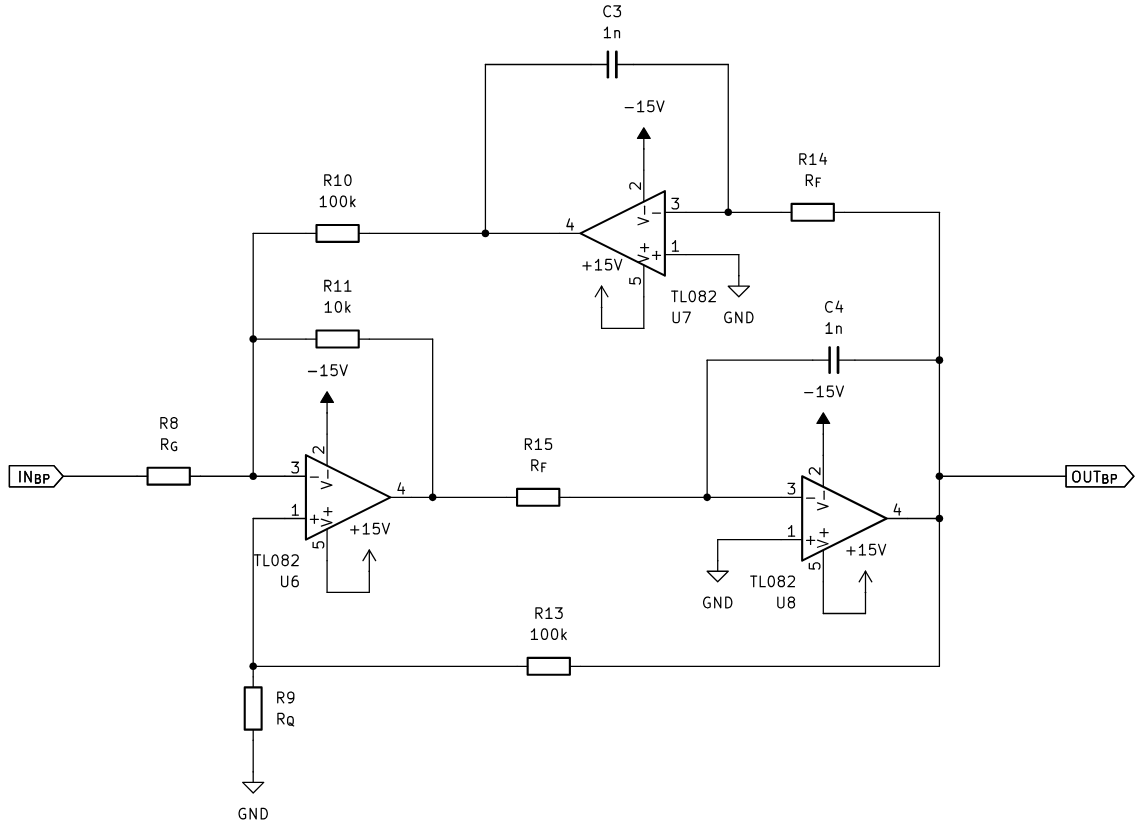
\includegraphics[width=0.8\textwidth]{stromlaufplan-bp.png}
    \caption{Topologie des für den Empfänger verwendeten Bandpassfilters \cite{horowitz_art_2015}}
    \label{fig:bandpass}
\end{figure}

\subsubsection{Berechnung des Filters}
In dem Buch \enquote{Art of Electronics}\cite{horowitz_art_2015} finden sich die Formeln~\eqref{eq:r_f},~\eqref{eq:r_q} und~\eqref{eq:r_g} für die Berechnung des in Abbildung~\ref{fig:bandpass} dargestellten Filters.
\begin{align}
    R_{\symup{F}} &= \frac{\num{5.03e7}}{f_{\symup{0}}} \label{eq:r_f}\\
    \vspace{1em}
    R_{\symup{Q}} &= \frac{\num{1e5}}{\num{3.48}Q + G - \num{1}} \label{eq:r_q}\\
    \vspace{1em}
    R_{\symup{G}} &= \num{3.16e4}\frac{Q}{G} \label{eq:r_g}
\end{align}

Der Wert \(Q\) berechnet sich nach Formel~\eqref{eq:q} aus der Mittenfrequenz und der Bandbreite.
\begin{equation}
    Q=\frac{f_{\symup{0}}}{B} \label{eq:q}
\end{equation}

Mit den vorgegebenen Werten ergibt sich \(R_{\symup{F}}=\qty{649.03}{\ohm}\), \(R_{\symup{Q}}=\qty{823.89}{\ohm}\) und \(R_{\symup{G}} = \qty{102.04}{\kilo\ohm}\). Damit ist der Filter vollständig berechnet.

\subsubsection{Verifizierung}
Zur Verifizierung wurde der Filter in KiCAD mit dem Operationsverstärker TL082 von Texas Instruments und den zuvor berechneten Werten aufgebaut, um den Amplitudengang zu simulieren. Die Simulationsergebnisse sind in Abbildung~\ref{fig:amplitudengang} dargestellt.
\begin{figure}
  \centering
  \begin{tikzpicture}
    \begin{semilogxaxis}[
      xlabel={Frequenz (Hz)},
      ylabel={Gain (dB)},
      title={Amplitudengang},
      grid=major,
      width=12cm,
      height=7cm,
      legend pos=south east,
    ]
      \addplot[
        blue,
        thick,
        smooth,
        mark=none,
      ] table[x index=0, y index=1, col sep=space] {data/amplitudengang_converted.txt};
      \addlegendentry{V(OUTBP)}
    \end{semilogxaxis}
  \end{tikzpicture}
  \caption{Amplitudengang des zuvor berechneten Filters}
  \label{fig:amplitudengang}
\end{figure}

Bei der Betrachtung des Amplitudengangs fällt auf, dass die Mittenfrequenz und auch der Filtergewinn vom erwarteten Ergebnis abweichen.
Die Abweichung der Verstärkung spielt keine größere Rolle.
Im Gegensatz dazu ist die Abweichung der Mittenfrequenz ein größeres Problem.
Um die Mittenfrequenz anzupassen wurde die \enquote{Tuned value} Funktion des Simulationstools in KiCAD verwendet, um die Werte der Widerstände so anzupassen, dass genau die Mittenfrequenz von \qty{77.5}{\kHz} getroffen wird.
Bei dieser Gelegenheit wurde die Verstärkung auf einen runden Wert von \qty{10}{\dB} angepasst.
Durch diese Simulation wurden die Werte \(R_{\symup{F}}= \qty{600}{\ohm}\), \(R_{\symup{Q}} = \qty{855}{\ohm}\) und \(R_{\symup{G}} = \qty{164}{\kilo\ohm}\) gefunden.

\subsection{weitere Verarbeitung des Signals}
\subsubsection{Verstärkung}
Das Signal sollte so verstärkt werden, dass es den Wertebereich des Analog-Digital-Wandlers voll ausschöpft. Um das zu erreichen kann ein Programmable Gain Amplifier, kurz PGA eingesetzt werden~\cite{d_engeler_performance_2012}.
Dieser ermöglicht es, die Verstärkung vom Digitalteil aus zu steuern, sodass der Wertebereich des Analog-Digital-Wandlers grundsätzlich voll ausgenutzt wird.
Da der Empfänger in diesem Beispiel nur an einem Ort benutzt werden soll, sodass sich die Empfangsstärke des Signals nicht wirklich ändert, kann der PGA auch durch eine einfache Operationsverstärkerschaltung ersetzt werden.
Hier soll ein nicht invertierender Verstärker, wie er in Abbildung~\ref{fig:amplifier} dargestellt ist, verwendet.
\begin{figure}[h!]
    \centering
    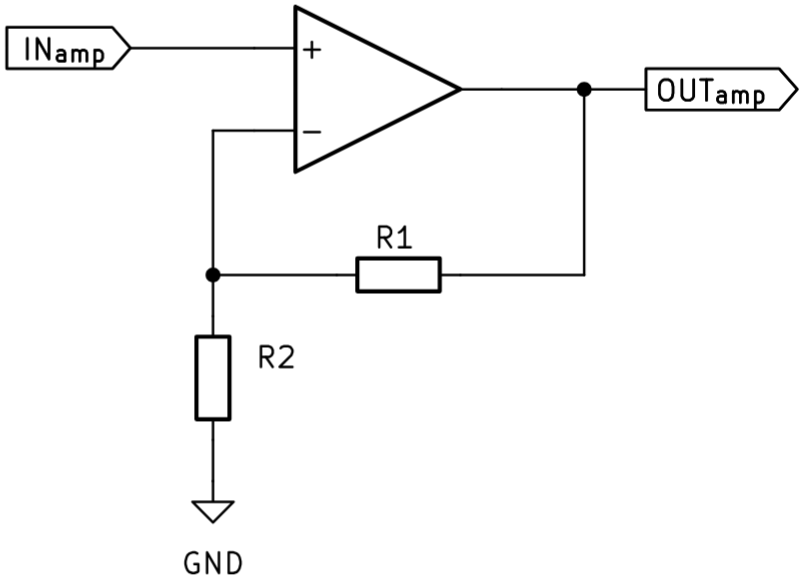
\includegraphics[width=0.8\textwidth]{amplifier}
    \caption{nicht invertierender Verstärker}
    \label{fig:amplifier}
\end{figure}
Dieser berechnet sich nach Formel~\eqref{eq:amp} und muss an die lokalen Empfangsbedingungen angepasst werden. Um ein bisschen mehr Flexibilität zu ermöglichen, kann statt mit festen Widerständen mit Potentiometern gearbeitet werden.
\begin{equation}
    V_{\symup{out}} = V_{\symup{in}} \cdot \left(1 + \frac{R_{\symup{1}}}{R_{\symup{2}}}\right) \label{eq:amp}
\end{equation}

\subsubsection{weitere Verarbeitung}
Das Signal könnte jetzt noch weiter analog demoduliert werden. Dazu könnte eine Diode in Verbindung mit einem RC-Tiefpass verwendet werden, um die Hüllkurve zu regenerieren, mit der die Trägerfrequenz moduliert wurde.
Dabei muss darauf geachtet werden, dass die Zeitkonstante zum einen nicht zu kurz gewählt wird, da so die Hüllkurve nicht vollständig regeneriert wird.
Zum Anderen darf die Zeitkonstante auch nicht zu lang gewählt werden, da dadurch die Flanken zu Beginn jeder Sekunde deutlich flacher werden und so die Möglichkeiten zur Detektion im Digitalteil eingeschränkt werden.
Das bedeutet jedoch zusätzlichen Hardware-Aufwand und einige zusätzliche Berechnungen.

Nachdem moderne Microcontroller über ADCs verfügen, die schnell genug sind, um die Trägerfrequenz von \qty{77.5}{\kHz} abzutasten.
Das Abtasttheorem von Shannon besagt, dass ein Signal mindestens mit der doppelten der größten in dem Signal enthaltenen Frequenz abgetastet werden muss, um eindeutig auf die ursprüngliche Signalform zurückführbar zu sein.
Dementsprechend muss die Abtastrate für das DCF77-Signal mindestens \(f_{\symup{s}} = 2 f_{\symup{c}} = \qty{155}{\kHz}\) betragen.
Die Microcontroller der STM32H7 Familie beispielsweise verfügen über drei 16-Bit ADCs, mit denen eine maximale Abtastrate von \qty{3.6}{\mega\samples} erreicht werden kann~\cite{stmicroelectronics_getting_2020}
Damit lässt sich das Abtasttheorem mit einem deutlichen Überhang erfüllen.
Durch diese Art der Weiterverarbeitung des verstärkten Signals, stehen zusätzlich zu den Pulsen auch die Informationen aus dem in Abschnitt~\ref{sec:modulation} angesprochenen Pseudo-Random-Noise Binary Phase Shift Keying zur Verfügung.

\section{Fazit}
Dieser Empfänger ist natürlich mehr ein Lernprojekt, als etwas, das man in einem kommerziellen Produkt verwenden würde.
Hier gibt es genug günstige Empfänger, die einfach verbaut werden können.
Außerdem stehen in der aktuellen Zeit viele weitere Möglichkeiten zur Zeitsynchronisation zur Verfügung. Einige Beispiele hierfür sind unter Anderem das Network-Time-Protokoll, kurz NTP und GPS, welches eine deutlich exaktere Synchronisation ermöglicht.
Dennoch bietet der Aufbau des Projektes die Möglichkeit, sich mit Antennen und deren Tuning, mit Verstärkern und analogen Filtern, sowohl aktiv als auch passiv zu beschäftigen.
\clearpage
\printbibliography
\end{document}
